%\documentclass[11pt,oneside,a4paper,openright]{report}
%\usepackage[utf8]{inputenc}
%\renewcommand{\contentsname}{Indholdsfortegnelse}
%\usepackage{pdfpages}
%\usepackage{titlesec}
%\titleformat{\chapter}{\normalfont\huge}{\thechapter.}{20pt}{\huge\it}

%%%% Dokumentklassen %%%%

\documentclass[a4paper,11pt,dvipsnames,oneside,openany]{memoir} 	% Openright åbner kapitler på højresider (openany begge)
% fleqn = flush left equation - sikre at alle ligninger tvinges til venstre. I 3. semesterprojektet, skulle ligningerne stå i midten derfor er denne pakke slettet fra dokumentklassen.

\usepackage{subfiles}
\usepackage{nameref}
\usepackage{tabularx}
\usepackage{multirow}
\usepackage[table]{xcolor}


%%%% PACKAGES %%%%

%% Oversættelse og tegnsætning %%
\usepackage[utf8]{inputenc}					% Input-indkodning af tegnsæt (UTF8)
\usepackage[danish]{babel}					% Dokumentets sprog
\usepackage[T1]{fontenc}				    % Output-indkodning af tegnsæt (T1)
\usepackage{ragged2e,anyfontsize}			% Justering af elementer
%\usepackage{fixltx2e}						% Retter forskellige fejl i LaTeX-kernen
\usepackage{titletoc}
\newcommand{\nocontentsline}[3]{}
\newcommand{\tocless}[2]{\bgroup\let\addcontentsline=\nocontentsline#1{#2}\egroup}									% Giver mulighed for at fjerne section nummer i indholdsfortegnelse ved \tocless


\usepackage{lastpage}						% Total antal sider opdateres automatisk ved \pageref{LastPage}
\usepackage{tikz}							% Til at lave flow diagrammer
\usetikzlibrary{calc,trees,positioning,arrows,chains,shapes.geometric,decorations.pathreplacing,decorations.pathmorphing,shapes,matrix,shapes.symbols}				% Til at lave diagrammer
																			
%% Figurer og tabeller (floats) %%
\usepackage{graphicx} 						% Håndtering af eksterne billeder (JPG, PNG, EPS, PDF)
\usepackage{multicol}         	           	% Muliggør output i spalter
\usepackage{rotating}						% Rotation af tekst med \begin{sideways}...\end{sideways}
\usepackage{xcolor}							% Definer farver med \definecolor. Se mere: http://en.wikibooks.org/wiki/LaTeX/Colors
\usepackage{flafter}						% Sørger for at floats ikke optræder i teksten før deres reference
\let\newfloat\relax 						% Justering mellem float-pakken og memoir
\usepackage{float}							% Muliggør eksakt placering af floats, f.eks. \begin{figure}[H]
\usepackage{color, colortbl}				% Tilføjer farve til tabeller

\definecolor{Gray}{gray}{0.9}				% Definerer en farve "yeezy-gray"

%% Matematik mm. %%
\usepackage{amsmath,amssymb,stmaryrd} 		% Avancerede matematik-udvidelser
\usepackage{mathtools}						% Andre matematik- og tegnudvidelser
\usepackage{textcomp}                 		% Symbol-udvidelser (fx promille-tegn med \textperthousand)
\usepackage{rsphrase}						% Kemi-pakke til RS-saetninger, fx \rsphrase{R1}
\usepackage[version=3]{mhchem} 				% Kemi-pakke til flot og let notation af formler, f.eks. \ce{Fe2O3}
\usepackage{siunitx}						% Flot og konsistent præsentation af tal og enheder med \si{enhed} og \SI{tal}{enhed}
\sisetup{output-decimal-marker = {,}}		% Opsætning af \SI (DE for komma som decimalseparator) 

%% Referencer og kilder %%
\usepackage[danish]{varioref}				% Muliggør bl.a. krydshenvisninger med sidetal (\vref)
\usepackage{natbib}							% Udvidelse med naturvidenskabelige citationsmodeller
\usepackage{xr}							    % Referencer til eksternt dokument med \externaldocument{<NAVN>}

%% Misc. %%
\usepackage{listings}						% Placer kildekode i dokumentet med \begin{lstlisting}...\end{lstlisting}
\usepackage{lipsum}							% Dummy text \lipsum[..]
\usepackage[shortlabels]{enumitem}			% Muliggør enkelt konfiguration af lister
\usepackage{pdfpages}						% Gør det muligt at inkludere pdf-dokumenter med kommandoen \includepdf[pages={x-y}]{fil.pdf}	
\pdfoptionpdfminorversion=6					% Muliggør inkludering af pdf-dokumenter, af version 1.6 og højere
\pretolerance=2500 							% Justering af afstand mellem ord (højt tal, mindre orddeling og mere luft mellem ord)


%%%% CUSTOM SETTINGS %%%%

%% Marginer %%
\setlrmarginsandblock{3.0cm}{3.0cm}{*}		% \setlrmarginsandblock{Indbinding}{Kant}{Ratio}
\setulmarginsandblock{3.0cm}{3.0cm}{*}		% \setulmarginsandblock{Top}{Bund}{Ratio}
\checkandfixthelayout 						% Oversætter værdier til brug for andre pakker

%% Afsnitsformatering %%
\setlength{\parindent}{0mm}           		% Størrelse af indryk
\setlength{\parskip}{3mm}          			% Afstand mellem afsnit ved brug af double Enter
\linespread{1,1}							% Linjeafstand

%% Indholdsfortegnelse %%
\setsecnumdepth{subsection}		 			% Dybden af nummererede overskrifter (part/chapter/section/subsection)
\maxsecnumdepth{subsection}					% Dokumentklassens grænse for nummereringsdybde
\settocdepth{subsubsection} 					% Dybden af indholdsfortegnelsen
\setcounter{secnumdepth}{5} 				    % Ekstra subsubsection nummerering
		
%% Opsætning af listings %%
\definecolor{commentGreen}{RGB}{34,139,24}
\definecolor{stringPurple}{RGB}{208,76,239}

\lstset{language=Matlab,				    % Sprog
	basicstyle=\ttfamily\scriptsize,	    % Opsætning af teksten
	keywords={for,if,while,else,elseif,		% Nøgleord at fremhæve
			  end,break,return,case,
			  switch,function},
	keywordstyle=\color{blue},				% Opsætning af nøgleord
	commentstyle=\color{commentGreen},		% Opsætning af kommentarer
	stringstyle=\color{stringPurple},		% Opsætning af strenge
	showstringspaces=false,					% Mellemrum i strenge enten vist eller blanke
	numbers=left, numberstyle=\tiny,		    % Linjenumre
	extendedchars=true, 					    % Tillader specielle karakterer
	columns=flexible,						% Kolonnejustering
	breaklines, breakatwhitespace=true,		% Bryd lange linjer
}

%% Navngivning %%
\addto\captionsdanish{
	\renewcommand\appendixname{Appendiks}
	\renewcommand\contentsname{Indholdsfortegnelse}	
	\renewcommand\appendixpagename{Appendiks}
	\renewcommand\appendixtocname{Appendiks}
	\renewcommand\cftchaptername{\chaptername~}		% Skriver "Kapitel" foran kapitlerne i indholdsfortegnelsen
	\renewcommand\cftappendixname{\appendixname~}	% Skriver "Appendiks" foran appendiks i indholdsfortegnelsen
}

%% Kapiteludssende %%
\definecolor{numbercolor}{gray}{0.7}		            % Definerer en farve til brug til kapiteludseende
\newif\ifchapternonum

\makechapterstyle{jenor}{					        % Definerer kapiteludseende frem til ...
  \renewcommand\beforechapskip{0pt}
  \renewcommand\printchaptername{}
  \renewcommand\printchapternum{}
  \renewcommand\printchapternonum{\chapternonumtrue}
  \renewcommand\chaptitlefont{\fontfamily{pbk}\fontseries{db}\fontshape{n}\fontsize{25}{35}\selectfont\raggedleft}
  \renewcommand\chapnumfont{\fontfamily{pbk}\fontseries{m}\fontshape{n}\fontsize{1in}{0in}\selectfont\color{numbercolor}}
  \renewcommand\printchaptertitle[1]{%
    \noindent
    \ifchapternonum
    \begin{tabularx}{\textwidth}{X}
    {\let\\\newline\chaptitlefont ##1\par} 
    \end{tabularx}
    \par\vskip-2.5mm\hrule
    \else
    \begin{tabularx}{\textwidth}{Xl}
    {\parbox[b]{\linewidth}{\chaptitlefont ##1}} & \raisebox{-15pt}{\chapnumfont \thechapter}
    \end{tabularx}
    \par\vskip2mm\hrule
    \fi
  }
}											        % ... her

\chapterstyle{jenor}						        % Valg af kapiteludseende - Google 'memoir chapter styles' for alternativer

%% Sidehoved %%

\makepagestyle{AAU}							        % Definerer sidehoved og sidefod udseende frem til ...
\makepsmarks{AAU}{%
	\createmark{chapter}{left}{shownumber}{}{. \ }
	\createmark{section}{right}{shownumber}{}{. \ }
	\createplainmark{toc}{both}{\contentsname}
	\createplainmark{lof}{both}{\listfigurename}
	\createplainmark{lot}{both}{\listtablename}
	\createplainmark{bib}{both}{\bibname}
	\createplainmark{index}{both}{\indexname}
	\createplainmark{glossary}{both}{\glossaryname}
}
\nouppercaseheads									% Ingen Caps ønskes

\makeevenhead{AAU}{\small E17BAC-Synk2}{}{\leftmark}	% Definerer lige siders sidehoved (\makeevenhead{Navn}{Venstre}{Center}{Hoejre})
\makeoddhead{AAU}{\rightmark}{}{}		            % Definerer ulige siders sidehoved (\makeoddhead{Navn}{Venstre}{Center}{Højre})
\makeevenfoot{AAU}{\small \thepage \ }{}{ }						% Definerer lige siders sidefod (\makeevenfoot{Navn}{Venstre}{Center}{Højre})
\makeoddfoot{AAU}{}{}{\small \thepage \ }						% Definerer ulige siders sidefod (\makeoddfoot{Navn}{Venstre}{Center}{Højre})

\copypagestyle{AAUchap}{AAU}							% Sidehoved for kapitelsider defineres som standardsider, men med blank sidehoved
\makeoddhead{AAUchap}{}{}{}
\makeevenhead{AAUchap}{}{}{}
\makeheadrule{AAUchap}{\textwidth}{0pt}
\aliaspagestyle{chapter}{AAUchap}					% Den ny style vælges til at gælde for chapters
													% ... her
															
\pagestyle{AAU}										% Valg af sidehoved og sidefod


%%%% CUSTOM COMMANDS %%%%

%% Billede hack %%
\newcommand{\figur}[4]{
		\begin{figure}[H] \centering
			\includegraphics[width=#1\textwidth]{billeder/#2}
			\caption{#3}\label{#4}
		\end{figure} 
}

%% Specielle tegn %%
\newcommand{\decC}{^{\circ}\text{C}}
\newcommand{\dec}{^{\circ}}
\newcommand{\m}{\cdot}


%%%% ORDDELING %%%%

\hyphenation{}


%%%% Tilføjelser af min preample %%%%

% Booktabs:
% The booktabs package is needed for better looking tables. 
\usepackage{booktabs}

% Caption:
% For better looking captions. See caption documentation on how to change the format of the captions.
\usepackage[hang, font={small, it}]{caption}

% Hyperref:
% This package makes all references within your document clickable. By default, these references will become boxed and colored. This is turned back to normal with the \hypersetup command below.
\usepackage{hyperref}
	\hypersetup{colorlinks=false,pdfborder=0 0 0}

% Cleveref:
% This package automatically detects the type of reference (equation, table, etc.) when the \cref{} command is used. It then adds a word in front of the reference, i.e. Fig. in front of a reference to a figure. With the \crefname{}{}{} command, these words may be changed.
\usepackage{cleveref}
	\crefname{equation}{formel}{formler}
	\crefname{figure}{figur}{figurer}	
	\crefname{table}{tabel}{tabeller}

% Mine tilføjelser:
\usepackage{units}                        %% Bruges til at gøre fx 1/2 samlet med: \nicefrac{1}{2}.
\usepackage{tabu, longtable}              %% Bruges til tabeller.
\setlength{\tabulinesep}{1.5ex}           %% Definerer linjeafstand i tabeller.
\usepackage{enumerate}                    %% Bruges til lister.
\usepackage{tabto}                        %% Giver mulighed for TAB med fx \tabto{3em}.
\usepackage[hyphenbreaks]{breakurl}       %% Bruges til websiders url'er.
\renewcommand{\UrlFont}{                  %% Definerer url-font.
\small\ttfamily}                          %
\bibliographystyle{unsrt}                 %% Definere bibliografien. Ses til sidst i dokumentet i kapitlet Litteratur.
\usepackage{amssymb} 
\usepackage{pifont}
%\newcommand{\xmark{\ding{55}}			 % Opretter et unchecked mark

\usepackage[bottom]{footmisc}

\usetikzlibrary{%
    decorations.pathreplacing,%
    decorations.pathmorphing,%
    arrows,
    arrows.meta,
    positioning,
    shapes,
    shadows,
    shapes.geometric
    }
    \usepackage{relsize}

%\definecolor{myblue1}{RGB}{0,157,209}
\definecolor{myblue1}{rgb}{0.12, 0.56, 1.0}
\definecolor{myblue3}{RGB}{216,229,245}
%\definecolor{myblue4}{RGB}{0,149,229}
\definecolor{myblue2}{rgb}{0.19, 0.55, 0.91}
\definecolor{myblue4}{rgb}{0.08, 0.38, 0.74}
\definecolor{myred1}{rgb}{0.82, 0.1, 0.26}
\definecolor{myyellow1}{rgb}{1.0, 0.96, 0.0}
\definecolor{myyellow2}{rgb}{1.0, 0.65, 0.0}


\usepackage{pdflscape}
\usepackage{rotating}

\begin{document}
\begin{titlingpage}
\begin{center}

~ \\[3cm]

%\includegraphics[width=0.6\textwidth]{figurer/ASE}~\\[1cm]

\textsc{\LARGE Bilag 8}\\[1.5cm]

%\textsc{\Large Sundhedsteknologi}\\
%\textsc{\Large 3. semesterprojekt}\\[0.5cm]

\noindent\makebox[\linewidth]{\rule{\textwidth}{0.4pt}}\\
[0.5cm]{\Huge Om Dysfagi}
\noindent\makebox[\linewidth]{\rule{\textwidth}{0.4pt}}
\end{center}
\vfill
\begin{center}
{\large 19. december 2017}
\end{center}
\end{titlingpage}

\newpage
\tableofcontents*
\newpage


\chapter{Om Dysfagi}
\section{Indledning}
En normal synkeproces forløber ved at mad og drikke passerer mundhulen, går forbi svælget inden processen fortsætter ned i spiserøret. Denne synkesprocess foregår ved, at bolus skubbes bagud mod svælget ved hjælp af tungen, som presser op og bagud. Derefter udløses en refleks pga. sanseceller i svælget. Dette foregår uden for viljens kontrol og i sammenspil med den forlængede rygmarv. Hele synkeprocessen er et samspil mellem 20-30 muskler, som enten skal trække sig sammen eller slappe af i den rigtige rækkefølge \cite{Sand2008}. 

Synkeprocessen består af fire sammenhængende faser:
\begin{enumerate}
\item Præ-Oral fase:\\
Denne fase indtræder forud for drikke- og fødeindtagelse  i munden. Den er karakteriset ved at spytproduktion og synkestimulation starter, når man ser og dufter til mad og drikke \cite [s. 12]{Kjaersgaard2013}.    
\item Oral fase (i munden): \\
I denne fase bliver maden bidt i stykker i munden. Her tygges maden, som bliver blandet med spyt og formet til en bolle (bolus). Ved hjælp af tungen transporteres bolus til den bagerste del af mundhulen samtidig med at ganespejlet lukker af op til næsen.
\item Faryngeale fase (i svælget): \\ Her bliver bolus transporteret gennem svælget og luftrøret beskyttes ved at stemmebåndet og strubelåget lukker samtidig med indgangen til spiserøret åbnes.     
\item Esophageal fase (i spiserøret):
Spiserøret indsnævres og bolus transporteres til mavesækken vha. en peristaltisk bevægelse \cite [s. 395]{Sand2008}.
\end{enumerate}

\begin{figure}[H]
\centering
{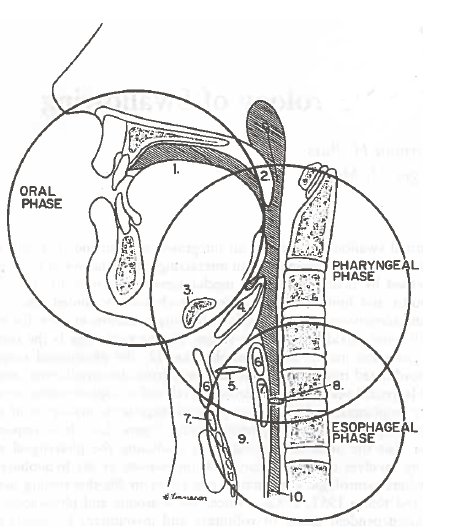
\includegraphics[width=6cm]
{Figure/dysfagi3faser}}
\caption{De tre sidste faser ved synkeprocessen\cite{Bass1992}}
\label{trefaser}
\end{figure}


\section{Definition af dysfagi?}
Dysfagi er den medicinske betegnelse for symptom relateret til dysfunktion af synkeprocessen \cite{KjaersgaardPh.d.studerende}. Dysfagi tilstanden er karakteriseret ved spise- og drikkevanskeligheder hos patienten. Resultatet kan være en fejlsynkning ved, at bolus ender i luftrøret i stedet for spiserøret. Dette kan bl.a. medføre udvikling af pneumoni.
\section{Hvem får dysfagi?}

Dysfagi symptomerne kan bl.a. observeres hos patienter med sklerose, apopleksi og parkinson.   Symptomerne forekommer også hos personer med kræft, KOL og almen svækkelse og aldring \cite{SallyRefsgaardTineOsterbyKristensen2015}. 

Ifølge patientombuddets temarapport fra 2012 om dysfagi at \cite{Bommersholdt2012}:

\begin{itemize}
\item 60-87 \% af beboere på plejehjem for ældre har synkebesværligheder.
\item 30 \% alle apopleksipatienter har dysfagi. 15.000 danskere rammes hvert år af apopleksi. Forekomsten af dysfagi er ca. 37-78 \% ved akut apopleksi. Hos patienter i den akutte fase, er dysfagi/aspiration en betydelig dødsårsag. Herudover lever 30-40.000 danskere med senfølger efter en apopleksi, nogle har dysfagi
\item 20-50 \% af patienter med Parkinson og Alzheimer har dysfagi. Der lever ca. 6. 000 patienter med Parkinson i Danamark og ca. 45.000 patienter med Alzheimer.  
\item 30-60 \% af patienter med muskelsvind har dysfagi.
\item Herudover er der ca. 10.000 børn, unge og voksne med Cerebral Parese (CP) også kendt som "spastisk lammelse", der har synkebesvær . 
\end{itemize}

\section{Konsekvenser}
Dysfagi kan have følgende konsekvenser \cite[s. 12]{KjaersgaardPh.d.studerende}:
\begin{itemize}
\item Manglende oral ernæring og dermed under- eller fejlernæring
\item Dehydrering
\item Aspiration
\item Kvælning
\item Udvikling af aspirationspneumoni
\item Social isolering
\item Øget risiko for mortalitet
\item Reduceret livskvalitet

\end{itemize}



\section{Nuværende håndtering af dysfagi}


Diagnosticering og udredning af øvre dysfagi kan inddeles i en tre-delt trin. Første trin  handler om at screene patientens mentale tilstand ved at vurdere patientens bevidsthedsniveau, orienteringsevne, handlekraft, samt evnen til at synke få konsistenstyper som vand og spytflåd. Hvis det vurderes af klinikeren, at der er behov for yderligere udredning, sendes patienten videre til en klinisk undersøgelse. Den kliniske undersøgelse er baseret på Facial-Oral-Tract-Therapy (F.O.T.T) metoden og anvendes til at vurdere parametre som patientens sensoriske og motoriske respons, åndedræt og oral indtagelse af fødebolus \cite[s. 23-25]{Kjaersgaard2013}. 

Den kliniske undersøgelse er præget af subjektive vurderinger, da det foretages af en klinikker uden hjælp af teknologiske apparater. Denne undersøgelsesmetode kan f.eks. overse silent aspiration, som kan medføre udvikling af pneumoni og i værste fald kvælning. Derfor anbefales det af sundhedsstyrelsens nationale kliniske retningslinjer for øvre dysfagi, at man supplere den kliniske undersøgelse med en instrumentel undersøgelse til voksne med synkebesvær \cite{Sundhedsstyrelsen2015}.

Den instrumentelle undersøgelse omfatter Fiber Endoskopisk Evaluering af Synkefunktionen (FEES) og/eller Funktionel Videoradiologisk Evaluering af Synkefunktionen (FVES).  Ved FEES undersøgelse, som er en invasiv intervention, fører klinikeren en fiberoptisk endoskop gennem patientens næse og pharynx for at få et visuelt billede af pharynx' anatomi. Anormaliteter, som observeres undervejs dokumenteres i en modificeret udgave af ”Der Berliner Dysphagia Index”, som er en standard protokol til dokumentation af FEES undersøgelse \cite{Lambertsen2007}. 

Undersøgelsen kan afdække patientens synkevanskeligheder ved at iagttage aspiration af bolus i luftvejene, tilstedeværelsen af bolus-rester i strubehovedet og patientens evne til at synke egen saliva \cite[s. 27-28]{Kjaersgaard2013}. 
Ved FVES undersøgelse anvendes røntgenstråler, som muliggør visualisering af fødebolus i alle faser. Klinikeren kan vha. denne metode evaluere om pharyngeal eller øsophageal muskler fungerer korrekt og om patienten kan kompensere for dysfagien med reflektoriske teknikker som fx ændring af hovedstilling. FEES og FVES anvendes som ”guld standarder” ved diagnosticering af patienter med øvre dysfagi, og begge undersøgelsesmetoder betragtes som komplementære værktøjer til udredning af dysfagi frem for konkurrerende \cite[s. 50]{Kjaersgaard2013}.



\bibliography{library}
\end{document}